\ifx\wholebook\relax \else

\documentclass[b5paper]{ctexart}
\usepackage[nomarginpar
  %, margin=.5in
]{geometry}

\addtolength{\oddsidemargin}{-0.05in}
\addtolength{\evensidemargin}{-0.05in}
\addtolength{\textwidth}{0.1in}

\usepackage[cn]{../prelude}

\setcounter{page}{1}

\begin{document}

\title{融合}

\author{刘新宇
\thanks{{\bfseries 刘新宇} \newline
  Email: liuxinyu95@gmail.com \newline}
  }

\maketitle
\fi

\markboth{融合}{编程中的数学}

\ifx\wholebook\relax
\chapter{融合}
\numberwithin{Exercise}{chapter}
\fi

\epigraph{3表示2+1,4表示3+1。所以接下来(虽然证明很长),4等于2+2。因此, 数学知识不再是神秘的。}{——罗素}

% ... mathematical knowledge ... is, in fact, merely verbal knowledge. "3" means "2+1", and "4" means "3+1". Hence it follows (though the proof is long) that "4" means the same as "2+2". Thus mathematical knowledge ceases to be mysterious.  -- Bertrand Russell

%\begin{wrapfigure}{R}{0.3\textwidth}
\begin{figure}[htbp]
 \centering
 \includegraphics[scale=0.5]{img/penrose-triangle}
 %\captionsetup{labelformat=empty}
 \caption{彭罗斯三角形}
 \label{fig:Penrose-triangle}
\end{figure}
%\end{wrapfigure}

记得在中学数学课上,老师会在黑板上写一个有很多字母的式子,然后让同学们化简。有人会自告奋勇站到讲台上,拿起粉笔在黑板上推导。合并同类项、因式分解……各种办法都可以用。这个过程就像是变魔术,最后往往得到意想不到的简单结果。当然也有卡住或者绕圈子的时候,老师总是耐心地提示,引导我们找到思路。这样的经历好像就发生在眼前,一方面,满手的粉笔灰让同学们体会到老师的不易,另一方面,那种推理的神秘强力量让我感到它的强大。我总是希望知道更多的公式,这样就能在化简或者推导时派上用场。这种推导的神奇之处在于,我们不用特别关心这些公式或者定理在当时场景下的具体含义。就像摆弄积木一样,从散落的各种零件,最后搭建起一个有趣玩具。这些公式和定理相互组装到一起,最后引向一个有趣的结果。看到$a^2 + 2ab + b^2$就会把它变换为$(a+b)^2$,就像把两块积木插到一起那样自然,我们不用在推导时强迫自己回想这个公式的几何意义。

\begin{figure}[htbp]
\centering
\begin{tikzpicture}
\draw[fill=gray, draw=black, pattern=north west lines]
  (0, 0) rectangle (4, 4);
\filldraw[fill=white]
  (0, 0) rectangle (1, 1)
  (1, 1) rectangle (4, 4);
\path (0.5, 0.5) node {$a^2$}
      (2.5, 2.5) node {$b^2$}
      (-0.5, 0.5) node {$a$}
      (2.5, 0.5) node {$ab$}
      (4.5, 2.5) node {$b$}
      (0.5, 2.5) node {$ab$};
\path (0, -1) node (l) {}
      (2, -1) node (m) {$a + b$}
      (4, -1) node (r) {};
\draw[->] (m) -- (l);
\draw[->] (m) -- (r);
\end{tikzpicture}
\caption{$(a + b)^2 = a^2 + 2ab + b^2$的几何意义}
\end{figure}

本章中,我们用两个例子说明如何进行编程中的推导。每个例子都既用直观方法也用推导方式给出解释。这就像$(a+b)^2$的情形。一方面我们可以用几何直观,将其理解为一大一小两个正方形和两个相等矩形的面积;另一方面,我们也可以用代数推导一步一步得出同样的结果。

\[
\begin{array}{rcll}
(a + b)^2 & = & (a + b)(a + b) & \text{二次方的定义} \\
          & = & a(a + b) + b(a + b) & \text{乘法分配律} \\
          & = & a^2 + ab + ba + b^2 & \text{再次用分配律} \\
          & = & a^2 + 2ab + b^2 & \text{合并同类项$ab$和$ba$}
\end{array}
\]

\section{叠加——构建的融合}

我们要举的第一个例子是叠加——构建的融合(foldr/build fusion law)。2015年Java在其1.8版本中加入了lambda表达式并且提供了一系列支持函数式编程的工具。但是有人很快发现,尽管一连串地函数调用表达能力很强,简洁优雅,但是性能会下降很多。原因之一就是这些串起来函数调用产生了大量中间结果。这些中间结果往往不是一两个简单的数值,而通常是列表、容器这样规模很大的结构。这些结构被下一个函数消费使用,然后就丢弃了。但是接下来会产生另一个同等规模的结构。这种产生——一次性消费——丢弃——再产生的过程,沿着函数调用链一环一环地重复,造成了计算的负担。例如,我们想判断一个列表中的每个元素是否都满足某个条件。可以这样进行定义\cite{GLPJ-1993}:

\[
all(p, xs) = and(map(p, xs))
\]

传入$all(prime, [2, 3, 5, 7, 11, 13, 17, 19, ...])$就可以判断列表中是否都是素数。但是这个实现的效率却不高。首先$map(prime, xs)$会产生一个和$xs$同样长度的列表,列表中的每个元素是一个布尔值[True, True, ...],每个布尔值表示对应的元素是不是素数。然后这个布尔值列表传入$and$函数,检查是否存在False。最后$xs$和布尔值列表都被丢弃,而仅仅返回一个布尔值作为最终结果。

下面是另一种定义,它能够避免产生中间的布尔值列表:

\[
\begin{array}{l}
all(p, xs) = h(xs) \\
  \begin{cases}
  h([\ ]) = True \\
  h(x:xs) = p(x) \land h(xs) \\
  \end{cases}
\end{array}
\]

虽然这个实现不产生中间结果,可是和前面的$and(map(p, xs)$比起来,既冗长又不直观。有没有什么办法,鱼和熊掌兼得,即不丧失直观性,又能避免低效的实现呢?我们发现有些变换满足这一要求。例如:

\[
map\ sqrt\  (map\ abs\ xs) = map\ (sqrt \circ abs)\ xs
\]

先把列表中每个元素取绝对值构成一列新数,然后再把这列数中的每个开方。这和把列表中每个数先取绝对值然后再立即开方后构成一列新数等价。由此我们可以得到一个转换规则:

\be
map\ f\ (map\ g\ xs) = map\ (f \circ g)\ xs
\ee

但是这样的规则太多了,我们无法全部把它们列出。并且在千变万化的程序中,我们无法一眼就看出应该用哪一条规则优化。吉尔(Gill)、朗奇布瑞(Launchbury)、佩顿$\cdot$琼斯(Peyton Jones)在1993年提出了一个方法,他们从列表最本质的构造和叠加操作入手,找到了优化的规律。

\subsection{列表的叠加操作}

我们在第一章就给出过列表的叠加操作,它的定义为:

\[
\begin{array}{l}
foldr\ \oplus\ z\ [\ ] = z \\
foldr\ \oplus\ z\ (x:xs) = x\ \oplus\ (foldr\ \oplus\ z\ xs) \\
\end{array}
\]

展开就是:

\be
foldr\ \oplus\ z\ [x_1, x_2, ..., x_n] = x_1 \oplus (x_2 \oplus (...(x_n \oplus z))...)
\ee

许多列表相关的操作都可以用叠加来定义。以下是一些典型的例子:

\begin{enumerate}
\item 累加:

\[
sum = foldr\ +\ 0
\]

\item 前面提到的$and$函数,计算一个布尔值列表中的所有元素的逻辑与:

\[
and = foldr\ \land\ True
\]

这是因为:

\[
and\ [x_1, x_2, ..., x_n] = x_1 \land (x_2 \land (...(x_n \land True))...)
\]

\item 在一个列表中查找某一个元素是否存在:

\[
elem\ x\ xs\ = foldr\ (a\ b \mapsto (a = x) \lor b)\ False\ xs
\]

\item 逐一映射:

\[
\begin{array}{rcl}
map\ f\ xs & = & foldr\ (x\ ys \mapsto f(x) : ys)\ [\ ]\ xs \\
           & = & foldr\ ((:) \circ f)\ [\ ]\ xs \\
\end{array}
\]

\item 用某一条件过滤列表中的元素:

\[
\begin{array}{rl}
filter\ p\ xs = foldr\ (x\ ys \mapsto
  \begin{cases}
    p(x): & x:ys\ \\
    \text{否则}: & ys
  \end{cases})\ [\ ]\ xs \\
\end{array}
\]

\item 两个列表连接:

\be
xs \doubleplus ys = foldr\ (:)\ ys\ xs
\label{eq:binary-concat}
\ee

这是因为:

\[
[x_1, x_2, ..., x_n] \doubleplus ys = x_1 : (x_2 : (...(x_n : ys))...)
\]

\item 多个列表连接:

\[
concat\ xss = foldr\ \doubleplus\ [\ ]\ xss
\]

\end{enumerate}

叠加操作是如此基本(上一章中,我们证明了叠加是列表的初始代数),如果我们能把列表的叠加操作的化简规律找到,就找到了所有列表操作的化简规律。

\subsection{叠加——构建融合律}
现在我们考虑,如果把空列表[\ ](即Nil)和连接操作“:”(即Cons)进行叠加会产生什么结果。

\be
foldr\ (:)\ [\ ]\ [x_1, x_2, ..., x_n] = x_1 : (x_2 : (...(x_n : [\ ]))...)
\label{eq:foldr-fixed-point}
\ee

这回我们得到了列表本身。你也许想到了上一章介绍的不动点,我们稍后会回到这个话题。换言之,如果我们有一个运算$g$,它能够从一个起始值,例如“[\ ]”,和一个二元组合运算,例如“:”,产生一个列表。我们可以定义这个列表构造过程$build$:

\be
build(g) = g((:), [\ ])
\label{eq:build-definition}
\ee

接着,如果用另一个起始值$z$和二元组合运算$f$,对这一列表进行叠加,其结果就相当于用$z$替换[\ ],用“$f$”替换“(:)”,然后直接调用过程$g$。

\be
\pmb{foldr}(f, z, \pmb{build}(g)) = g(f, z)
\ee

写成无参数括号的形式就是:

\be
\pmb{foldr}\ f\ z\ (\pmb{build}\ g) = g\ f\ z
\label{eq:foldr-build-fusion-law}
\ee

\index{叠加——构建融合}
我们称这一结果为\textbf{叠加——构建融合定律}。

在继续深入介绍前,让我们先看一些具体的例子。考虑如何计算从$a$到$b$间的整数和$sum([a, a+1, ..., b-1, b])$。为此我们可以先产生从$a$到$b$之间的所有整数$a, a+1, a+2, ..., b-1, b$,例如使用下面的方法:

\[
range(a, b) =
\begin{cases}
a > b: & [\ ] \\
\text{否则}: & a : range(a+1, b) \\
\end{cases}
\]

这样$range(1, 5)$就产生列表[1, 2, 3, 4, 5]。接下来只要把这个列表中的元素累加起来就得到答案了:

\[
sum(range(a, b))
\]

接下来关键的一步,我们把$range$中的起始值[\ ]和二元组合运算(:)抽出成为参数,分别叫做$z$和$\oplus$:

\[
range'(a, b, \oplus, z) =
  \begin{cases}
  a > b: & z \\
  \text{否则}: & a \oplus range'(a+1, b, \oplus, z) \\
  \end{cases}
\]

我们甚至可以把$range'$的后两个参数柯里化:

\[
range'\ a\ b = \oplus\ z \mapsto
  \begin{cases}
  a > b: & z \\
  \text{否则}: & a\ \oplus\ (range'\ (a+1)\ b\ \oplus\ z) \\
  \end{cases}
\]

这样原来的$range$就可以用$range'$和$build$表示了:

\[
range(a, b) = build(range'(a, b))
\]

接下来我们用融合律化简累加和的计算:

\[
\begin{array}{rcll}
sum(range(a, b)) & = & sum(build(range'(a, b))) & \text{代入} \\
  & = & \pmb{foldr}\ (+)\ 0\ (\pmb{build}\ (range'\ a\ b)) & \text{用叠加表示累加} \\
  & = & range'\ a\ b\ (+)\ 0 & \text{使用融合律} \\
\end{array}
\]

这样就完成了化简,避免产生了中间列表,优化了算法。我们可以看一下最后的效果:

\[
range'\ a\ b\ (+)\ 0 =
  \begin{cases}
  a > b: & 0 \\
  \text{否则}: & a + (range'\ (a+1)\ b\ (+)\ 0) \\
  \end{cases}
\]

\subsection{列表的构建形式}

为了方便使用融合律,我们可以把常见的列表生成操作写为$build...foldr$的形式。这样当用叠加操作和$build...foldr$形式组合起来时:$\pmb{foldr}...(\pmb{build}...foldr)$,就可以使用融合律化简。

\begin{enumerate}
\item 首先是最简单的操作——构造空列表:

\[
[\ ]= build\ (f\ z \mapsto z)
\]

我们可以代入$build$的定义\cref{eq:build-definition}来验证这个定义:

\begin{proof}
\bre
build\ (f\ z \mapsto z) & = & (f\ z \mapsto z)\ (:)\ [\ ] & build\text{的定义} \\
  & = & (:)\ [\ ] \mapsto [\ ] & \beta-\text{规约,参见第二章} \\
  & = & [\ ] & \\
\ere
\end{proof}

\item 接下来是列表的链接(Cons)操作:

\[
x : xs = build\ (f\ z \mapsto f\ x\ (foldr\ f\ z\ xs))
\]

\begin{proof}
\blre
  & build\ (f\ z \mapsto f\ x\ (foldr\ f\ z\ xs)) & \\
= & (f\ z \mapsto f\ x\ (foldr\ f\ z\ xs))\ (:)\ [\ ] & build\text{的定义} \\
= & x : (foldr\ (:)\ [\ ]\ xs) & \beta-\text{规约} \\
= & x : xs & \text{由\cref{eq:foldr-fixed-point},叠加的不动点} \\
\elre
\end{proof}

\item 然后是列表的连接:

\[
xs \doubleplus ys = build\ (f\ z \mapsto foldr\ f\ (foldr\ f\ z\ ys)\ xs)
\]

\begin{proof}
\blre
  & build\ (f\ z \mapsto foldr\ f\ (foldr\ f\ z\ ys) xs) & \\
= & (f\ z \mapsto foldr\ f\ (foldr\ f\ z\ ys)\ xs)\ (:)\ [\ ] & build \text{的定义} \\
= & foldr\ (:)\ (foldr\ (:)\ [\ ]\ ys)\ xs & \beta-\text{规约} \\
= & foldr\ (:)\ ys\ xs & \text{对内层用叠加的不动点} \\
= & xs \doubleplus ys & \text{由\cref{eq:binary-concat},列表的连接} \\
\elre
\end{proof}

\end{enumerate}

以下操作我们只列出结果,而把它们的证明作为本小节的练习。

\begin{enumerate}
\setcounter{enumi}{3}
\item 多个列表的连接:
\[
concat\ xss = build\ (f\ z \mapsto foldr\ (xs\ x \mapsto foldr\ f\ x\ xs)\ z\ xss)
\]

\item 一一映射产生新列表:

\[
map\ f\ xs = build\ (\oplus\ z \mapsto foldr\ (y\ ys \mapsto (f\ y) \oplus ys)\ z\ xs)
\]

\item 过滤元素产生新列表:

\[
filter\ p\ xs = build\ (\oplus\ z \mapsto foldr\ (x\ xs' \mapsto
  \begin{cases}
    p(x): & x \oplus xs' \\
    \text{否则}: & xs' \\
  \end{cases})\ z\ xs) \\
\]

\item 重复产生同一元素的(无穷)列表:

\[
repeat\ x = build\ (\oplus\ z \mapsto let\ r = x \oplus r\ in\ r)
\]

\end{enumerate}

\subsection{使用融合律化简}

接下来我们使用刚刚打造好的融合律来化简计算。首先是本节开始时举过的例子:$all(p, xs) = and(map(p, xs))$

\begin{example}
我们把$and$改为叠加形式,把$map$改为构建形式就可以进行化简了。

\bea{cll}
  & all(p, xs) \\
= & and(map(p, xs)) & \text{原始定义} \\
= & foldr\ \land\ True\ map(p, xs) & and\text{的叠加形式} \\
= & \pmb{foldr}\ \land\ True\ \pmb{build}\ (\oplus\ z \mapsto & \\
  & \quad \quad foldr\ (x\ ys \mapsto p(x) \oplus ys)\ z\ xs) & map\text{的构建形式} \\
= & (\oplus\ z \mapsto foldr\ (x\ ys \mapsto p(x) \oplus ys)\ z\ xs)\ \land\ True & \text{融合律} \\
= & foldr\ (x\ ys \mapsto p(x) \land ys)\ True\ xs & \beta-\text{规约} \\
\eea

如果定义一个$first$函数,它将一个函数$f$应用到一对值中的前一个上,即:

\[
(first\ f)\ x\ y = f(x)\ y
\]

这样就可以进一步化简为:

\[
all\ p = foldr\ (\land) \circ (first\ p)\ True
\]

\end{example}

\begin{example}
我们举的第二个例子是把若干词语添加上空格,然后连接成句子。这样的文字处理过程通常叫做$join$,简单起见,我们在句子最后也添上一个空格。一个典型的定义如下:

\[
join(ws) = concat(map(w \mapsto w \doubleplus ['\ '], ws))
\]

这个定义简单直观,它先用逐一映射,在每个单词的末尾添加空格,得到一个新的单词列表,然后再把这个列表连接成一个字符串。但是这个定义的性能不佳。在单词末尾添加空格是一个昂贵的计算,需要先移动到每个单词的末尾,然后再使用字符串连接操作。其次有多少单词,逐一映射就会产生多长的新列表。最后这些中间结果都被丢弃了。接下来我们用融合律优化这一计算。

\[ \begin{array}{rl}
  & join(ws) \\
  & \{\text{定义} \} \\
= & concat(map(w \mapsto w \doubleplus ['\ '], ws)) \\

  & \{\text{把$concat$写为构建形式}\} \\
= & build\ (f\ z \mapsto \\
  & \quad foldr\ (x\ y \mapsto foldr\ f\ y\ x)\ z\ map(w \mapsto w \doubleplus ['\ '], ws)) \\

  & \{\text{把$map$写为构建形式}\} \\
= & build\ (f\ z \mapsto \\
  & \quad \pmb{foldr}\ (x\ y \mapsto foldr\ f\ y\ x)\ z\ (\pmb{build}\ (f'\ z' \mapsto \\
  & \quad \quad foldr\ (w\ b \mapsto f'\ (w \mapsto w \doubleplus ['\ '])\ b)\ z'\ ws))) \\
\end{array}
\]
\[ \begin{array}{rl}
  & \{\text{融合律}\} \\
= & build\ (f\ z \mapsto \\
  & \quad foldr\ (w\ b \mapsto (x\ y \mapsto foldr\ f\ y\ x)\ (w \doubleplus ['\ '])\ b)\ z\ ws) \\

  & \{\beta-\text{规约}x, y\} \\
= & build\ (f\ z \mapsto \\
  & \quad foldr\ (w\ b \mapsto foldr\ f\ b\ (w \doubleplus ['\ ']))\ z\ ws) \\

  & \{\text{把$\doubleplus$写为构建形式}\} \\
= & build\ (f\ z \mapsto \\
  & \quad foldr\ (w\ b \mapsto \\
  & \quad \quad \pmb{foldr}\ f\ b\ (\pmb{build}\ (f'\ z' \mapsto \\
  & \quad \quad \quad foldr\ f'\ (foldr\ f'\ z'\ ['\ '])\ w)))\ z\ ws) \\
\end{array}
\]
\[ \begin{array}{rl}
  & \{\text{融合律}\} \\
= & build\ (f\ z \mapsto \\
  & \quad foldr\ (w\ b \mapsto \\
  & \quad \quad foldr\ (foldr\ f\ b\ ['\ '])\ w)\ z\ ws) \\

  & \{\text{据$build$的定义,将$(:)$和$[\ ]$代入}\} \\
= & foldr\ (w\ b \mapsto foldr\ (:)\ \pmb{(foldr\ (:)\ b\ ['\ '])}\ w)\ [\ ]\ ws \\

  & \{\text{对黑体字部分求值}\} \\
= & foldr\ (w\ b \mapsto foldr\ (:)\ ('\ ' : b)\ w)\ [\ ]\ ws \\
\end{array} \]

因此最后化简的结果为:

\[
join(ws) = foldr\ (w\ b \mapsto foldr\ (:)\ ('\ ' : b)\ w)\ [\ ]\ ws
\]

我们还可以据此把叠加操作展开,得到一个可读性和性能都好的定义:

\[
\begin{array}{l}
\begin{cases}
join\ [\ ] = [\ ] \\
join\ (w:ws) = h\ w \\
\end{cases} \\
\text{其中}: \begin{cases}
             h\ [\ ] = '\ ' : join\ ws \\
             h\ (x:xs) = x : h\ xs \\
             \end{cases} \\
\end{array}
\]

\index{concatMap} \index{flatMap}
未经简化的$join$定义中使用了$concat \circ map(f)$这种组合,它十分常见,很多编程环境的标准库已经提供了这样的优化实现。\footnote{例如Haskell中的\texttt{concatMap},Java和Scala中的\texttt{flatMap}。}
\end{example}

第二个例子虽然展示了融合律的强大,但是也暴露出了一个问题。推导过程机械繁琐、容易出错。这恰恰是机器,而非人类擅长的事情。有些编程环境,例如Haskell已经把融合律实现在编译器内部\cite{GLPJ-1993}。这样只要我们把列表的常见操作用构建——叠加形式定义好,机器就可以替代我们利用融合律进行上述化简,从而得到优化的程序,避免中间结果和多余的递归\footnote{例如Haskell标准库已经用构建——叠加形式实现了大多数列表操作。}。随着时间的推移,更多的编译器会逐渐支持这一优化工具。

\subsection{类型限制}

每当我们打造出抽象的工具,就要思考它的适用范围,了解它什么情况下会失效。对于融合律也是如此。考虑下面的矛盾结果:

\blre
  & \pmb{foldr}\ f\ z\ (\pmb{build}\ (c\ n \mapsto [0])) & \\
= & (c\ n \mapsto [0])\ f\ z & \text{融合律} \\
= & [0] & \beta-\text{规约} \\
\elre

另一方面:

\blre
  & foldr\ f\ z\ (build\ (c\ n \mapsto [0])) & \\
= & foldr\ f\ z\ ((c\ n \mapsto [0])\ (:)\ [\ ]) & build\text{的定义} \\
= & foldr\ f\ z\ [0] & \beta-\text{规约} \\
= & f(0, z) & \text{叠加展开} \\
\elre

显然$f(0, z)$不等于$[0]$,连它们两个的类型都不同\footnote{除非特殊情况$f = (:), z = [\ ]$。}。造成这一矛盾结果的原因是$(c\ n \mapsto [0])$不是一个真正用$c$和$n$构造出结果的函数。为此我们需要对融合律$foldr\ f\ z\ (build\ g) = g\ f\ z$中$g$的类型做出限制。它的第一个参数既可以接受$c$,也可以接受$f$,换言之,它接受一个多态的二元运算$\forall A. \forall B.\ A \times B \to B$;同理它的第二个参数也是一个多态类型$B$的起始值,并产生一个类型为$B$的结果。我们把二元运算写为柯里化的形式就得到:

\[
g : \forall A. (\forall B. (A \to B \to B) \to B \to B)
\]

容易看出,上面反例中的类型是:$\forall A. (\forall B. (A \to B \to B) \to B \to [Int])$。不满足我们的类型限制。与此对应,构建函数$build$的类型为:

\[
build : \forall A. (\forall B. (A \to B \to B) \to B \to B) \to \mathbf{List}\ A
\]

\index{二阶多态函数}
由于里面有两个多态的类型$A$和$B$,因此它被称为二阶多态函数(rank-2 type polymorphic)。

\subsection{用范畴论推导融合律}
\index{短路融合(shortcut fusion)}
叠加——构建融合律可以用范畴理论推导出来并进行扩展。一旦把范畴论作为理论工具,人们就发现叠加——构建融合仅仅是众多种融合规则中的一个。现在这些规则统一被称为“短路融合”(shortcut fusion)。它们在编译器优化,程序库优化中发挥了重要的作用。我们无法在这一章中对它们做全面的介绍。读者可以参考\cite{Hinze-Harper-James-2010}深入了解短路融合的理论和实践方法。

在上一章中,我们介绍了F-代数,特别是初始代数和向下态射。由于初始代数是起始对象,所以它到任何其他代数都有唯一的箭头。如下图所示:

\begin{center}
\begin{tikzpicture}
  \matrix (m) [matrix of math nodes,
               row sep=3em, column sep=3em, minimum width=2em]{
    \mathbf{F} I  & I \\
    \mathbf{F} A  & A \\};
  \path[-stealth]
    (m-1-1) edge node [above] {$i$} (m-1-2)
    (m-1-1) edge node [left] {$\mathbf{F} \lbb a \rbb$} (m-2-1)
    (m-1-2) edge node [right] {$\lbb a \rbb$}  (m-2-2)
    (m-2-1) edge node [below] {$a$} (m-2-2);
\end{tikzpicture}
\end{center}

从初始代数$(I, i)$到另一代数$(A, a)$的箭头可以通过向下态射$\lbb a \rbb$来表示。如果还存在一个不同的F-代数$(B, b)$对象,并且有从$A$到$B$的箭头$A \arrowto{h} B$,就可以在范畴图下方把$(B, b)$也画出:

\begin{center}
\begin{tikzpicture}
  \matrix (m) [matrix of math nodes,
               row sep=3em, column sep=3em, minimum width=2em]{
    \mathbf{F} I & I \\
    \mathbf{F} A & A \\
    \mathbf{F} B & B \\};
  \path[-stealth]
    (m-1-1) edge node [above] {$i$} (m-1-2)
    (m-1-1) edge node [left] {$\mathbf{F} \lbb a \rbb$} (m-2-1)
    (m-1-2) edge node [right] {$\lbb a \rbb$}  (m-2-2)
    (m-2-1) edge node [below] {$a$} (m-2-2)
    (m-3-1) edge node [below] {$b$} (m-3-2)
    (m-2-1) edge node [left] {$\mathbf{F}(h)$} (m-3-1)
    (m-2-2) edge node [right] {$h$} (m-3-2);
\end{tikzpicture}
\end{center}

由于$(I, i)$是起始对象,所以它到$(B, b)$也必然存在唯一的箭头。由此可知,必然存在从$I$到$B$的箭头,可以用向下态射$\lbb b \rbb$表示出来。如下图:

\begin{center}
\begin{tikzpicture}
  \matrix (m) [matrix of math nodes,
               row sep=3em, column sep=3em, minimum width=2em]{
    \mathbf{F} I & I & \\
    \mathbf{F} A & A & \lbb b \rbb \\
    \mathbf{F} B & B & \\};
  \path[-stealth]
    (m-1-1) edge node [above] {$i$} (m-1-2)
    (m-1-1) edge node [left] {$\mathbf{F} \lbb a \rbb$} (m-2-1)
    (m-1-2) edge node [right] {$\lbb a \rbb$}  (m-2-2)
    (m-2-1) edge node [below] {$a$} (m-2-2)
    (m-3-1) edge node [below] {$b$} (m-3-2)
    (m-2-1) edge node [left] {$\mathbf{F}(h)$} (m-3-1)
    (m-2-2) edge node [right] {$h$} (m-3-2);
  \draw[-stealth]
    (m-1-2) .. controls (m-2-3) .. (m-3-2);
\end{tikzpicture}
\end{center}

从这个范畴图可以看出,当且仅当存在$h$,使得下面那个小正方形可交换,则从$I$经由$A$到$B$相当于从$I$直接到$B$。这就是初始代数的融合律。记为:

\be
\begin{array}{rcl}
A \arrowto{h} B \Rightarrow h \circ \lbb a \rbb = \lbb b \rbb
& \iff &
h \circ a = b \circ \mathbf{F}(h) \\
\end{array}
\ee

初始代数的融合律意味着什么呢?在上一章中,我们发现向下态射可以将非递归的计算,转换成在递归结构上的叠加计算。例如,当函子$\mathbf{F}$是$\mathbf{ListF}A$(其中$A$是给定的对象)时,箭头$a = f + z$,而初始箭头$i = (:) + [\ ]$,向下态射$\lbb a \rbb = foldr(f, z)$。如果记$b = c + n$,则融合律可以写成:

\[
h \circ foldr(f, z) = foldr(c, n)
\]

它说明叠加之后再进行变换可以化简为单一的叠加。1995年,高野秋彦和梅耶(Meijer)进一步将向下态射$\lbb a \rbb$抽象成从$a$构造某种代数结构$g\ a$,这样融合律就可以推广为\cite{Takano-Meijer-1995}:

\be
A \arrowto{h} B \quad \Rightarrow \quad h \circ g\ a = g\ b
\ee

\index{酸雨定律} \index{砍伐定律(deforestation)}
这一推广的融合律被称为“酸雨定律”\footnote{由于融合律能够消除不必要的中间结果,所以最早被称为“砍伐定律”(deforestation)。而推广的融合律被幽默地称为酸雨定律(acid rain law)。}。另一方面,由于存在从初始代数$I$到$A$的箭头:$I \arrowto{\lbb a \rbb} A$,所以将$\lbb a \rbb$代入酸雨定律左侧的$h$,并且用$i$替换酸雨定律中的$a$,用$a$替换酸雨定律中的$b$,我们有:

\be
I \arrowto{\lbb a \rbb} A \quad \Rightarrow \quad \lbb a \rbb \circ g\ i = g\ a
\ee

具体到列表的例子,把$\lbb a \rbb$代换为$foldr(f, z)$;把初始代数$i$代换为列表的初始代数$(:) + [\ ]$;定义$build(g) = g\ (:)\ [\ ]$,并代入酸雨定律左侧,就得到了列表的叠加——构建融合律:

\blre
& \lbb a \rbb \circ g\ i = g\ a & \text{酸雨定律} \\

\Rightarrow &
foldr\ f\ z\ (g\ i) = g\ a & \text{列表的向下态射是叠加} \\

\Rightarrow &
foldr\ f\ z\ (g\ (:)\ [\ ]) = g\ a & \text{列表的初始代数$i$是$(:), [\ ]$} \\

\Rightarrow &
foldr\ f\ z\ (g\ (:)\ [\ ]) = g\ f\ z & \text{用$f, z$替换$a$} \\

\Rightarrow &
\pmb{foldr}\ f\ z\ (\pmb{build}\ g) = g\ f\ z & \text{反向用$build$的定义} \\
\elre

这样我们就用范畴论证明了叠加——构建融合律\cite{Hinze-Harper-James-2010}。

\begin{Exercise}\label{ex:fusion-law}
\Question{验证左侧叠加也可以表示为$foldr$:
\[
foldl\ f\ z\ xs = foldr\ (b\ g\ a \mapsto g\ (f\ a\ b))\ id\ xs\ z
\]}
\Question{证明以下列表的构建——叠加形式:
\[
\resizebox{\linewidth}{!}{\ensuremath{
\begin{array}{l}
concat\ xss = build\ (f\ z \mapsto foldr\ (xs\ x \mapsto foldr\ f\ x\ xs)\ z\ xss) \\
map\ f\ xs = build\ (\oplus\ z \mapsto foldr\ (y\ ys \mapsto (f\ y) \oplus ys)\ z\ xs) \\
filter\ p\ xs = build\ (\oplus\ z \mapsto foldr\ (x\ xs' \mapsto
  \begin{cases}
     p(x): & x \oplus xs' \\
    \text{否则}: & xs' \\
  \end{cases})\ z\ xs) \\
repeat\ x = build\ (\oplus\ z \mapsto let\ r = x \oplus r\ in\ r) \\
\end{array}
}}
\]
}
\Question{化简快速排序算法:
\[
\resizebox{\linewidth}{!}{\ensuremath{
\begin{cases}
qsort\ [\ ] = [\ ] \\
qsort\ (x:xs) = qsort\ [a | a \in xs, a \leq x] \doubleplus [x] \doubleplus qsort\ [a | a \in xs, x < a] \\
\end{cases}
}}
\]
提示:将ZF表达式\footnote{全称为“策梅罗——弗兰克尔表达式”。指集合论中$\{f(x) | x \in X, p(x), q(x), ...\}$这样的集合构建表达式。我们在下一章介绍无穷和集合论时会再次遇到它。}转换为$filter$。}
\Question{利用范畴论验证融合律的类型限制。提示:考虑向下态射的类型。}
\end{Exercise}

\begin{Answer}[ref = {ex:fusion-law}]
\Question{验证左侧叠加也可以表示为$foldr$:
\[
foldl\ f\ z\ xs = foldr\ (b\ g\ a \mapsto g\ (f\ a\ b))\ id\ xs\ z
\]

为了方便理解,我们将其改写为:

\[\begin{array}{l}
foldl\ f\ z\ xs = foldr\ step\ id\ xs\ z \\
\text{其中:} step\ x\ g\ a = g\ (f\ a\ x)
\end{array}\]

\[
\resizebox{\linewidth}{!}{\ensuremath{
\begin{array}{cll}
  & foldl\ f\ z\ [x_1, x_2, ..., x_n] \\
= & (foldr\ step\ id\ [x_1, x_2, ..., x_n])\ z \\
= & (step\ x_1 (step\ x_2 ( ... (step\ x_n\ id))) ...)\ z \\
= & (step\ x_1 (step\ x_2 ( ... (a_n \mapsto id\ (f\ a_n\ x_n)))) ...)\ z \\
= & (step\ x_1 (step\ x_2 ( ...(a_{n-1} \mapsto (a_n \mapsto id\ (f\ a_n\ x_n))\ (f\ a_{n-1}\ x_{n-1}))))...)\ z \\
= & (a_1 \mapsto (a_2 \mapsto ( ... (a_n \mapsto id\ (f\ a_n\ x_n))\ (f\ a_{n-1}\ x_{n-1})) ... (f\ a_2\ x_2)) (f\ a_1\ x_1))\ z \\
= & (a_1 \mapsto (a_2 \mapsto ( ... (a_n \mapsto f\ a_n\ x_n)\ (f\ a_{n-1}\ x_{n-1})) ... )\ (f\ a_1\ x_1))\ z \\
= & (a_1 \mapsto (a_2 \mapsto (... (a_{n-1} \mapsto f\ (f\ a_{n-1}\ x_{n-1})\ x_n)\ ...))\ (f\ a_1\ x_1))\ z \\
= & (a_1 \mapsto f\ (f\ (...(f\ a_1\ x_1)\ x_2)\ ...)\ x_n)\ z \\
= & f\ (f\ (...(f\ z\ x_1)\ x_2)\ ...)\ x_n
\end{array}
}}
\]

如果把$f$改写成$\oplus$,并写成中缀形式,就能看出$foldl$和$foldr$的区别:

\[
foldl\ \oplus\ f\ z = ((...(z \oplus x_1)\ \oplus x_2)...)\ \oplus x_n
\]
}
\Question{证明以下列表的构建——叠加形式:
\[
\begin{array}{l}
concat\ xss = build\ (f\ z \mapsto foldr\ (xs\ x \mapsto foldr\ f\ x\ xs)\ z\ xss) \\
map\ f\ xs = build\ (\oplus\ z \mapsto foldr\ (y\ ys \mapsto (f\ y) \oplus ys)\ z\ xs) \\
filter\ p\ xs = build\ (\oplus\ z \mapsto foldr\ (x\ xs' \mapsto
  \begin{cases}
     p(x): & x \oplus xs' \\
    \text{否则}: & xs' \\
  \end{cases})\ z\ xs) \\
repeat\ x = build\ (\oplus\ z \mapsto let\ r = x \oplus r\ in\ r) \\
\end{array}
\]

首先是多个列表的连接$concat$
\begin{proof}
\[
\resizebox{\linewidth}{!}{\ensuremath{
\begin{array}{cll}
  & build\ (f\ z \mapsto foldr\ (xs\ x \mapsto foldr\ f\ x\ xs)\ z\ xss) \\
= & (f\ z \mapsto foldr\ (xs\ x \mapsto foldr\ f\ x\ xs)\ z\ xss)\ (:)\ [\ ] & \text{$build$的定义} \\
= & foldr\ (xs\ x \mapsto foldr\ (:)\ x\ xs)\ [\ ]\ xss & \text{$\beta$-规约} \\
= & foldr\ \doubleplus [\ ]\ xss & \text{两个列表连接的定义} \\
= & concat\ xss & \text{多列表连接的定义} \\
\end{array}
}}
\]
\end{proof}

接着是逐一映射$map$
\begin{proof}
\blre
  & build\ (\oplus\ z \mapsto foldr\ (y\ ys \mapsto (f\ y) \oplus ys)\ z\ xs) \\
= & (\oplus\ z \mapsto foldr\ (y\ ys \mapsto (f\ y) \oplus ys)\ z\ xs)\ (:)\ [\ ] & \text{$build$的定义} \\
= & foldr\ (y\ ys \mapsto f(y) : ys)\ [\ ]\ xs & \text{$\beta$-规约} \\
= & foldr\ (x\ ys \mapsto f(x) : ys)\ [\ ]\ xs & \text{$\alpha$变换,改名字} \\
= & map\ f\ xs & \text{逐一映射的定义} \\
\elre
\end{proof}

接着是过滤操作$filter$

\begin{proof}
\[
\resizebox{\linewidth}{!}{\ensuremath{
\begin{array}{cll}
  & build\ (\oplus\ z \mapsto foldr\ (x\ xs' \mapsto
  \begin{cases}
     p(x): & x \oplus xs' \\
    \text{否则}: & xs' \\
  \end{cases})\ z\ xs) \\
= & (\oplus\ z \mapsto foldr\ (x\ xs' \mapsto
  \begin{cases}
     p(x): & x \oplus xs' \\
    \text{否则}: & xs' \\
  \end{cases})\ z\ xs)\ (:)\ [\ ] & \text{$build$的定义} \\
= & foldr\ (x\ xs' \mapsto
  \begin{cases}
     p(x): & x : xs' \\
    \text{否则}: & xs' \\
  \end{cases})\ [\ ]\ xs & \text{$\beta$-规约} \\
= & filter\ p\ xs & \text{过滤操作的定义} \\
\end{array}
}}
\]
\end{proof}

最后是重复操作$repeat$

\begin{proof}
\blre
  & build\ (\oplus\ z \mapsto let\ r = x \oplus r\ in\ r) \\
= & (\oplus\ z \mapsto let\ r = x \oplus r\ in\ r)\ (:)\ [\ ] & \text{$build$的定义} \\
= & (let\ r = x : r\ in\ r) & \text{$\beta$-规约} \\
= & repeat\ x & \text{重复操作的定义} \\
\elre
\end{proof}
}
\Question{化简快速排序算法:
\[
\resizebox{\linewidth}{!}{\ensuremath{
\begin{cases}
qsort\ [\ ] = [\ ] \\
qsort\ (x:xs) = qsort\ [a | a \in xs, a \leq x] \doubleplus [x] \doubleplus qsort\ [a | a \in xs, x < a] \\
\end{cases}
}}
\]

可以把ZF表达式变换成$filter$。显然这里处理了两遍列表,它们可以合成一次:

\[
\begin{cases}
qsort\ [\ ] & = [\ ] \\
qsort\ (x:xs) & = qsort\ as \doubleplus [x] \doubleplus qsort\ bs \\
\end{cases}
\]

其中:
\[\begin{array}{l}
(as, bs) = foldr\ h\ ([\ ], [\ ])\ xs \\
h\ y\ (as', bs') = \begin{cases}
               y \leq x : & (y:as', bs') \\
               \text{否则}: & (as', y:bs') \\
\end{cases} \\
\end{array}\]

接下来我们可以把两个列表的连接操作化简:

\blre
  & qsort\ as \doubleplus [x] \doubleplus qsort\ bs \\
= & qsort\ as \doubleplus (x : qsort\ bs) \\
= & foldr (:)\ (x : qsort\ bs) (qsort\ as)
\elre
}
\Question{利用范畴论验证融合律的类型限制。提示:考虑向下态射的类型。

观察范畴图:

\begin{center}
\begin{tikzpicture}
  \matrix (m) [matrix of math nodes,
               row sep=3em, column sep=5em, minimum width=2em]{
     \mathbf{ListF} A\ \lbrack A \rbrack & \lbrack A \rbrack \\
     \mathbf{ListF} A\ B\ & B \\};
  \path[-stealth]
    (m-1-1) edge node [left] {$\mathbf{ListF} A(h)$} (m-2-1)
    (m-1-2) edge node [right] {$h = \lbb \alpha \rbb$} (m-2-2)
    (m-1-1) edge node [above] {$(:) + [\ ]$} (m-1-2)
    (m-2-1) edge node [below] {$\alpha = f + z$} (m-2-2);
\end{tikzpicture}
\end{center}

向下态射$\lbb \alpha \rbb$被抽象成从$\alpha$构造某种代数结构$g\ \alpha$。$g$接受一个$F$-代数的$\alpha$箭头,产生结果$B$。$\alpha$箭头是$f : A \to B \to B$和$z : 1 \to B$的和。故其类型为:

\[
g : \forall A. (\forall B. (A \to B \to B) \to B \to B)
\]

构造的定义是$build(g) = g\ (:)\ [\ ]$,它把$g$应用到初始代数的$\alpha$箭头上从而构造出初始代数中的对象,也就是列表$[A]$。因而:

\[
build : \forall A. (\forall B. (A \to B \to B) \to B \to B) \to \mathbf{List}\ A
\]
}
\end{Answer}

\section{巧算100}

我们举的第二个例子来自伯德的《函数式算法珠玑》中的第6章\cite{Bird-2010}。高德纳在《计算机程序设计的艺术》卷4中给出了一道练习题\cite{Knuth-TAOCP-2006}:把1到9这九个数字写成一行:1 2 3 4 5 6 7 8 9。只允许在这些数字之间添上加号和乘号,不许用括弧。如何使得最后的得数恰好是100?

例如:

\[
12 + 34 + 5 \times 6 + 7 + 8 + 9 = 100
\]

这看起来像是一道小学生的数学谜题。如果要求找到所有可能的解法,就是一道编程趣题。最简单直接的方法,就是利用计算机进行穷举,每两个数字间一共有三种选择:1)什么都不插入;2)插入加号;3)插入乘号。由于九个数字间一共有8个空,所以共有$3^8 = 6561$种方法。我们只要让计算机逐一检查这6561种方案,看看哪些最终得100就可以了。

\subsection{穷举法}

我们先把一个由数字、加法、乘法组成的式子定义出来。考虑算式:

\[
12 + 34 + 5 \times 6 + 7 + 8 + 9
\]

由于先乘除后加减,我们可以把它看作由加号分割的若干子算式,即:

\[
sum\ [12, 34, 5 \times 6, 7, 8, 9]
\]

我们定义由加号分割的若干子算式$t_1 + t_2 + ... + t_n$为$expr = [t_1, t_2, ..., t_n]$:

\lstset{frame = single}
\begin{Haskell}
type Expr = [Term]
\end{Haskell}

具体到每个子算式,我们可以把它看作由乘号分割的若干因子,例如$5 \times 6 = product\ [5, 6]$。如果是单一的数,例如$34$,我们仍然可以把它看作$34 = product\ [34]$。这样我们就可以定义由因子组成的子算式$f_1 \times f_2 \times ... \times f_m$。即$term = [f_1, f_2, ..., f_m]$:

\begin{Haskell}
type Term = [Factor]
\end{Haskell}

最终,每个因子都可以看作若干数字组成的整数,例如由两个数字组成的34,或仅有一个数字的5。也就是说$\textit{factor} = [d_1, d_2, ..., d_k]$:

\begin{Haskell}
type Factor = [Int]
\end{Haskell}

从若干数字求得整数是一个叠加的过程,例如$[1, 2, 3] \Rightarrow (((1 \times 10) + 2) \times 10) + 3$。我们可以将其定义为一个函数:

\[
dec = foldl\ (n\ d \mapsto n \times 10 + d)\ 0
\]

穷举法的思路是针对每一个可能的算式,计算并检查它是否得100。为此,我们需要定义一个函数,求出一个算式的值。根据算式的定义,我们需要递归地求出每个子算式(term)的值,然后将其累加起来;为了求每个子算式的值,需要递归地求出每个因子的值,然后再累乘起来;为了求每个因子的值,需要对每个因子使用$dec$函数。

\[
eval = sum \circ map\ (product \circ (map\ dec))
\]

明显这一定义可以用上一节介绍的融合律进行优化,我们把具体的推导过程留作练习。最终的优化结果如下:

\[
eval = foldr\ (t\ ts \mapsto (foldr\ ((\times) \circ fork(dec, id))\ 1\ t) + ts)\ 0
\]

其中$fork(f, g)\ x = (f\ x, g\ x)$,它将两个函数分别应用到一个变量上,然后将结果组成一对值。从这一结果可以写出一个可读性与性能都更好的定义:

\[
\begin{cases}
eval\ [\ ] = 0 \\
eval (t:ts) = product\ (map\ dec\ t) + eval(ts) \\
\end{cases}
\]

根据这一定义,如果算式为空,则其值为0;否则我们取出第一个子算式,将其中的每个因子求出并乘到一起。然后再加上剩余子算式的求值结果。这样在使用穷举法时,对每个可能的算式,我们都用$eval$求值。留下所有等于100的算式。即:

\[
filter\ (e \mapsto eval(e) == 100)\ es
\]

其中$es$是所有从1到9能够组成的算式的集合。如何产生这个集合呢?我们从空集开始,然后每次从1到9中取出一个数字,看看能扩展出哪些合法的算式。首先,从空集和唯一的数字$d$只能构造出一个算式:$[[[d]]]$。最内层是由数字$d$构成的唯一因子$fact = [d]$;然后是由这个因子构成的子算式$term = [fact] = [[d]]$,这个唯一的子算式构成的完整算式是$[term] = [[fact]] = [[[d]]]$。我们可以把这一构造过程定义为:

\[
expr(d) = [[[d]]]
\]

接下来,考虑一般情形。我们的策略是从右侧开始,不断取出数字9, 8, 7, ...来扩展算式。假设我们已经用数字构造了一个算式集合$[e_1, e_2, ..., e_n]$,此时如果取出下一个数字$d$,如何扩展出所有的合法算式呢?我们在本节的开头说过,每两个数字间一共由三种选择:1)什么都不插入;2)插入加号;3)插入乘号。我们来看看对于算式集合中的任意$e_i$这三种选择的含义分别是什么。将$e_i$展开表示成若干子算式的和$e_i = t_1 + t_2 + ...$,其中第一个子算式$t_1$表示为若干因子的积$t_1 = f_1 \times f_2 \times ...$。

\begin{enumerate}
\item 什么都不插入意味着将数字$d$直接添加到$e_i$的第一个子算式中的第一个因子的前面。这样由$d:f_1$组成一个新的因子。例如$e_i$是算式$8 + 9$,数字$d$是7,将7写在$8+9$的前面而什么符号都不插入,这样就得到新算式$78 + 9$;
\item 插入乘号意味着用数字$d$构成一个因子$[d]$,然后将它添加到$e_i$中第一个子算式的前面。这样由$[d]:t_1$组成一个新的子算式。具体到$8 + 9$这个例子,我们把7写在它的前面,然后在7和8之间插入一个乘号,这样就得到新算式$7 \times 8 + 9$;
\item 插入加号意味着用数字$d$构成一个子算式$[[d]]$,然后将将它添加到$e_i$的最前面,组成新的算式$[[d]]:e_i$。具体到$8 + 9$这个例子,我们把7写在它的前面,然后在7和8之间插入一个加号,这样就得到新算式$7 + 8 + 9$。
\end{enumerate}

把这三种情形转换为定义就得到了下面的函数:

\begin{Haskell}
add d ((ds:fs):ts) = [((d:ds):fs):ts,
                      ([d]:ds:fs):ts,
                      [[d]]:(ds:fs):ts]
\end{Haskell}

其中算式$e_i$被写成了$(ds:fs):ts$的形式,$e_i$中的第一个子算式是$ds:fs$,第一个子算式中的第一个因子是$ds$。这样,从每个已有的算式,我们都可以扩展出3个新算式。而对于算式列表$[e_1, e_2, ..., e_n]$,只要分别对每个算式扩展,然后将结果连接到一起就可以了。这恰恰就是上一节我们介绍过的\textit{concatMap}:

\[
\begin{cases}
extend\ d\ [\ ] = [expr(d)] \\
extend\ d\ es = \textit{concatMap}\ (add\ d)\ es
\end{cases}
\]

这样我们就得到了穷举法的完整定义:

\be
filter\ (e \mapsto eval(e) == 100)\ (foldr\ extend\ [1..9])
\label{eq:puzzle100-basic}
\ee

\subsection{改进}

我们能改进这个穷举法么?观察用1到9这些数字从右向左穷举算式的过程。首先我们写下数字9,在添加数字8时,可能产生3个算式,分别是:89,$8 \times 9 = 72$,和8 + 9 = 17。接下来添加7,算式789显然大于100,可以立即丢弃。并且我们确信任何在789左侧扩展出的新算式也都不可能等于100,因此也可以丢弃。这样就避免了无谓的计算。同样$7 \times 89$也大于100,可以丢弃并停止向左扩展。只有7+89是可能的候选算式。接下来我们扩展出$78 \times 9$,由于它大于100,因此被丢弃并停止扩展……

通过这一过程,我们发现,可以一边扩展算式,一边计算当前算式的值。只要超过100就丢弃并停止从这一候选算式向左继续扩展。整个过程就像一棵不断生长的树,只要树枝代表的算式超过100,就砍掉树枝,停止这一分支的生长。

\begin{figure}[htbp]
\centering
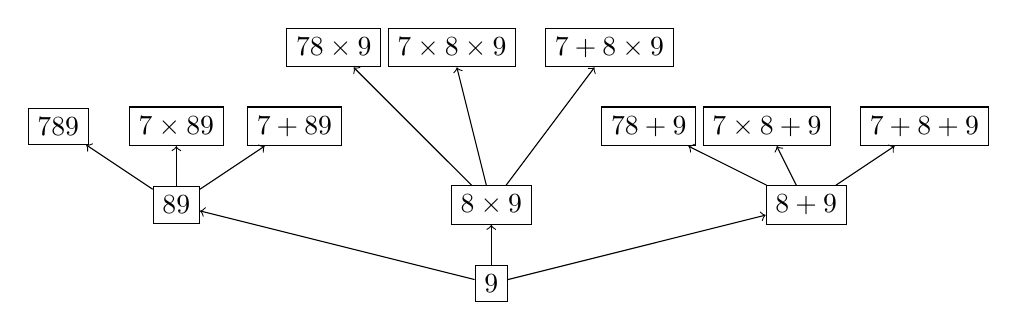
\begin{tikzpicture}
\path (0, 0)  node[rectangle, draw] (9) {9}
      (-4, 1) node[rectangle, draw] (89) {89}
      (0, 1)  node[rectangle, draw] (8x9) {$8 \times 9$}
      (4, 1)  node[rectangle, draw] (8+9) {$8 + 9$}
      (-5.5, 2) node[rectangle, draw] (789) {\sout{789}}
      (-4, 2) node[rectangle, draw] (7x89) {\sout{$7 \times 89$}}
      (-2.5, 2) node[rectangle, draw] (7+89) {$7 + 89$}
      (-2, 3) node[rectangle, draw] (78x9) {\sout{$78 \times 9$}}
      (-0.5, 3)  node[rectangle, draw] (7x8x9) {\sout{$7 \times 8 \times 9$}}
      (1.5, 3)  node[rectangle, draw] (7+8x9) {$7 + 8 \times 9$}
      (2, 2)  node[rectangle, draw] (78+9) {$78 + 9$}
      (3.5, 2)  node[rectangle, draw] (7x8+9) {$7 \times 8 + 9$}
      (5.5, 2)  node[rectangle, draw] (7+8+9) {$7 + 8 + 9$};
\draw[->] (9) edge (89)
          (9) edge (8x9)
          (9) edge (8+9)
          (89) edge (789)
          (89) edge (7x89)
          (89) edge (7+89)
          (8x9) edge (78x9)
          (8x9) edge (7x8x9)
          (8x9) edge (7+8x9)
          (8+9) edge (78+9)
          (8+9) edge (7x8+9)
          (8+9) edge (7+8+9);
\end{tikzpicture}
\caption{穷举算式的过程类似一棵生长的树}
\end{figure}

为了能够一边扩展算式,一边快速计算当前算式的值,我们可以将算式的值分离成三个部分:第一个子算式中的第一个因子的值$f$,除去$f$外剩余因子的乘积$v_{fs}$,以及除去第一个子算式外,剩余所有子算式的和$v_{ts}$。有了这三个部分,我们就可以计算出整个算式的值$f \times v_{fs} + v_{ts}$。

此时,如果继续向左扩展一个数字$d$,对应三种选择,算式及其值的更新分别如下:

\begin{enumerate}
\item 不插入任何符号,将$d$添加到第一个因子前作为最高位数字。算式的值等于:$(d \times 10^{n+1} + f) \times v_{fs} + v_{ts}$,其中$n$是因子$f$的位数。因此值的三个部分更新为:$f' = d \times 10^{n+1} + f$,$v_{fs}$和$v_{ts}$保持不变。
\item 插入乘号,将$d$作为第一个子算式中的第一个因子。算式的值等于:$d \times f \times v_{fs} + v_{ts}$。因此值的三个部分更新为:$f' = d, v_{fs'} = f \times v_{fs}$,$v_{ts}$不变。
\item 插入加号,将$d$作为新的第一个子算式。算式的值等于:$d + f \times v_{fs} + v_{ts}$。因此值的三个部分更新为:$f' = d, v_{fs'} = 1, v_{ts'} = f \times v_{fs} + v_{ts}$。
\end{enumerate}

为了方便第一条中$10^{n+1}$的计算,我们可以把指数也记录下来作为算式值的第四个部分。这样算式的值就可以表示为一个四元组$(e, f, v_{fs}, v_{ts})$。从四元组计算算式值的定义为:

\be
value(e, f, v_{fs}, v_{ts}) = f \times v_{fs} + v_{ts}
\ee

这样在扩展算式时,我们可以一边扩展,一边更新四元组,并将结果成对放在一起:

\be
\begin{array}{rrl}
add & d\ (((ds:fs):ts), & (e, f, v_{fs}, v_{ts})) = \\
&  [(((d:ds):fs):ts, & (10 \times e, d \times e + f, v_{fs}, v_{ts})), \\
&   (([d]:ds:fs):ts, & (10, d, f \times v_{fs}, v_{ts})), \\
&   ([[d]]:(ds:fs):ts, & (10, d, 1, f \times v_{fs} + v_{ts}))] \\
\end{array}
\ee

对于每一对算式和四元组,我们利用$value$函数,将四元组的值求出,如果大于100就立即丢弃,停止对其继续扩展。然后将候选算式和四元组对连接成一个列表。根据这一思路,我们将之前定义的$extend$重新定义为:

\be
\resizebox{0.9\linewidth}{!}{\ensuremath{
\begin{cases}
expand\ d\ [\ ] = [(expr(d), (10, d, 1, 0))] \\
expand\ d\ evs = \textit{concatMap}\ ((filter\ ((\leq 100) \circ value \circ snd)) \circ (add\ d))\ evs\\
\end{cases}
}}
\ee

现在我们可以对$expand$进行叠加,从1到9扩展出所有小于等于100的候选算式和四元组。最后我们计算四元组的值,然后选出所有恰好等于100的算式。

\be
map\ fst \circ filter\ ((=100) \circ value \circ snd)\ (foldr\ expand\ [\ ]\ [1, 2, ..., 9])
\ee

在本章附录中,我们给出了根据这一定义编写的程序。下面列出了等于100的所有7个算式:

\[
\begin{array}{rl}
1: & 1 \times 2 \times 3 + 4 + 5 + 6 + 7 + 8 \times 9 \\
2: & 1 + 2 + 3 + 4 + 5 + 6 + 7 + 8 \times 9 \\
3: & 1 \times 2 \times 3 \times 4 + 5 + 6 + 7 \times 8 + 9 \\
4: & 12 + 3 \times 4 + 5 + 6 + 7 \times 8 + 9 \\
5: & 1 + 2 \times 3 + 4 + 5 + 67 + 8 + 9 \\
6: & 1 \times 2 + 34 + 5 + 6 \times 7 + 8 + 9 \\
7: & 12 + 34 + 5 \times 6 + 7 + 8 + 9 \\
\end{array}
\]

\begin{Exercise}\label{ex:make-centry}
\Question{利用融合律化简算式求值的定义
\[
eval = sum \circ map\ (product \circ (map\ dec))
\]}
\Question{如何从左侧扩展出所有的算式?}
\Question{下面定义可以将算式翻译为字符串:
\[
str = (join\ \text{``+''}) \circ (map\ ((join\ \text{``} \times \text{''}) \circ (map\ (show \circ dec))))
\]
其中$show$可以将数字转换为字符串。函数 $join(c, s)$ 将一组字符串$s$用$c$连接起来,例如 $join($``\#''$, [$``abc'', ``def''$]) = $``abc\#def'' 。利用融合律化简$str$的定义。
}
\end{Exercise}

\begin{Answer}[ref = {ex:make-centry}]
\Question{利用融合律化简算式求值的定义$eval = sum \circ map\ (product \circ (map\ dec))$。

\[
%\resizebox{\linewidth}{!}{\ensuremath{
\begin{array}{cll}
  & eval\ es \\
  & \{ \text{函数组合} \} \\
= & sum (map\ (product \circ (map\ dec))\ es) \\
  & \{ \text{$sum$展开为叠加形式,$map$展开为构建形式} \} \\
= & \pmb{foldr}\ (+)\ 0\ (\pmb{build}\ (\oplus\ z\ \mapsto foldr\ (t\ ts \mapsto (f\ t) \oplus ts)\ z\ es)) \\
  & \{ \text{令$f = product \circ (map\ dec)$,并用融合律} \}\\
= & (\oplus\ z \mapsto foldr\ (t\ ts \mapsto (f\ t) \oplus ts)\ z\ es)\ (+)\ 0 \\
  & \{ \text{$\beta$-规约} \} \\
= & foldr\ (t\ ts \mapsto (f\ t) + ts)\ 0\ es \\
\end{array}
%}}
\]

写成无参数形式就是:

\[
eval = foldr\ (t\ ts \mapsto (f\ t) + ts)\ 0
\]

接下来我们再化简$product \circ (map\ dec)$部分

\[
%\resizebox{\linewidth}{!}{\ensuremath{
\begin{array}{cll}
  & (product \circ (map\ dec))\ t \\
  & \{ \text{函数组合} \} \\
= & product\ (map\ dec\ t) \\
  & \{ \text{$product$展开为叠加形式,$map$展开为构建形式} \} \\
= & \pmb{foldr}\ (\times)\ 1\ (\pmb{build}\ (\oplus\ z \mapsto foldr\ (d\ ds \mapsto (dec\ d) \oplus ds)\ z\ t)) \\
  & \{ \text{融合律} \} \\
= & (\oplus\ z \mapsto foldr (d\ ds \mapsto (dec\ d) \oplus ds)\ z\ t)\ (\times)\ 1 \\
  & \{ \text{$\beta$-规约} \} \\
= & foldr\ (d\ ds \mapsto (dec\ d) \times ds)\ 1\ t \\
  & \{ \text{定义$fork(f, g)\ x = (f\ x, g\ x)$} \} \\
= & foldr\ ((\times) \circ fork\ (dec, id))\ 1\ t \\
\end{array}
%}}
\]

接着把这个结果代入之前的$f$,得到最终化简的结果:

\[
eval = foldr\ (t\ ts \mapsto (foldr\ ((\times) \circ fork\ (dec, id))\ 1\ t) + ts)\ 0
\]
}
\Question{如何从左侧扩展出所有的算式?

从左向右扩展时,针对每个数字$d$,有三种选择:

\begin{enumerate}
\item 什么都不插入意味着将数字$d$直接添加到$e_i$的最后一个子算式中的最后一个因子的后面。这样由$f_n \doubleplus [d]$组成一个新的因子。例如$e_i$是算式$1 + 2$,数字$d$是3,将3写在$1 + 2$的后面而什么符号都不插入,这样就得到新算式$1 + 23$;
\item 插入乘号意味着用数字$d$构成一个因子$[d]$,然后将它添加到$e_i$中最后一个子算式的后面。这样由$t_m \doubleplus [[d]]$组成一个新的子算式。具体到$1 + 2$这个例子,我们把3写在它的后面,然后在2和3之间插入一个乘号,这样就得到新算式$1 + 2 \times 3$;
\item 插入加号意味着用数字$d$构成一个子算式$[[d]]$,然后将将它添加到$e_i$的最后面,组成新的算式$e_i \doubleplus [[[d]]]$。具体到$1 + 2$这个例子,我们把3写在它的后面,然后在2和3之间插入一个加号,这样就得到新算式$1 + 2 + 3$。
\end{enumerate}

为了将一个元素加到序列的末尾,我们可以定义一个函数:

\[
append\ x = foldr\ (:)\ [x]
\]

然后我们定义一个函数$onLast(f)$,它把$f$应用到一个序列的最后一个元素上:

\[\begin{array}{l}
onLast\ f = foldr\ h\ [\ ] \\
\text{其中}: \begin{cases}
  h\ x\ [\ ] & = [(f\ x)] \\
  h\ x\ xs & = x : xs \\
\end{cases} \\
\end{array}\]

然后,我们就可以实现这3种情况的扩展:

\begin{Haskell}
add d exp = [((append d) `onLast`) `onLast` exp,
             (append [d]) `onLast` exp,
             (append [[d]]) exp]
\end{Haskell}
}
\Question{下面定义可以将算式翻译为字符串:
\[
str = (join\ \text{``+''}) \circ (map\ ((join\ \text{``} \times \text{''}) \circ (map\ (show \circ dec))))
\]
其中$show$可以将数字转换为字符串。函数 $join(c, s)$ 将一组字符串$s$用$c$连接起来,例如 $join($``\#''$, [$``abc'', ``def''$]) = $``abc\#def'' 。利用融合律化简$str$的定义。

第五章中,我们给出了$join(ws)$的结果,它实际上是用空格分割一组字符串。将空格作为参数,就得到了$join(c, s)$的定义:

\[
join\ c = foldr\ (w\ b \mapsto foldr\ (:)\ (c:b)\ w)\ []
\]

观察$str$的定义,它实际上是两重的$(join\ c) \circ (map\ f)$的形式,即:

\[\begin{array}{l}
str = (join\ c) \circ (map\ f) \\
\text{其中}: f = (join\ d) \circ (map\ g) \\
\end{array}\]

这里$c =$ `+',$d =$ `$\times$',而$g = show \circ dec$。为此我们只要找出$(join\ c) \circ (map\ f)$的简化形式就可以了。

\[
\resizebox{\linewidth}{!}{\ensuremath{
\begin{array}{cll}
  & (join\ c) \circ (map\ f)\ es \\
  & \{ \text{$join$展开为叠加,$map$展开为构建形式} \} \\
= & \pmb{foldr}\ (w\ b \mapsto foldr\ (:) (c:b)\ w)\ [\ ]\ (\pmb{build}\ (\oplus\ z \mapsto foldr\ (y\ ys \mapsto (f\ y) \oplus ys)\ z\ es)) \\
  & \{ \text{融合律} \} \\
= & (\oplus\ z \mapsto foldr\ (y\ ys \mapsto (f\ y) \oplus ys)\ z\ es))\ (w\ b \mapsto foldr\ (:)\ (c:b)\ w)\ [\ ] \\
  & \{ \text{$\beta$-规约} \} \\
= & foldr\ (y\ ys \mapsto foldr\ (:)\ (c:ys)\ (f\ y))\ [\ ]\ es \\
\end{array}
}}
\]

将之前的加号、乘号,以及$show \circ dec$代入,我们得到结果:

\blre
str & = & foldr\ (x\ xs \mapsto foldr\ (:)\ (`+':xs) ( \\
    &   & \quad foldr (y\ ys \mapsto foldr\ (:)\ (`\times':ys)\ (show \circ dec\ y))\ [\ ])\ [\ ] \\
\elre
}
\end{Answer}

\section{小结和扩展阅读}

程序推导是数学推导的一种特殊情况。通过这一手段,我们可以从直观的、未经化简或优化的定义出发,利用一套形式化的方法和定理,一步一步进行变换。从而最终得到简洁的、优化的结果。伯德在他的《函数式算法设计珠玑》\cite{Bird-2010}中给出了很多例子。程序推导的正确性根植于数学。为此需要一套完整的理论,能够将计算机程序形式化、数学化,而不是仅仅依赖于人的直觉。抽象代数和范畴理论正是帮助我们对计算机编程进行形式化的强大工具。叠加——构建融合律就是这样的一个典型的例子。在1993年的论文\cite{GLPJ-1993}中,人们发现了系统化简程序的一个工具。随着范畴理论的引入,一系列融合律被发展出来\cite{Hinze-Harper-James-2010},并应用于计算机程序的推导和优化。

\section{附录代码}

Haskell中的\texttt{build}和\texttt{concatMap}定义:

\begin{Haskell}
build :: forall a. (forall b. (a -> b -> b) -> b -> b) -> [a]
build g = g (:) []

concatMap f xs = build (\c n -> foldr (\x b -> foldr c b (f x)) n xs)
\end{Haskell}

用穷举法巧算100的基本定义:
\begin{Haskell}[mathescape = true]
type Expr = [Term]     -- $T_1 + T_2 + ... T_n$
type Term = [Factor]   -- $F_1 \times F_2 \times ... F_m$
type Factor = [Int]    -- $d_1 d_2 ...d_k$

dec :: Factor -> Int
dec = foldl (\n d -> n * 10 + d) 0

expr d = [[[d]]]  -- single digit expr

eval [] = 0
eval (t:ts) = product (map dec t) + eval ts

extend :: Int -> [Expr] -> [Expr]
extend d [] = [expr d]
extend d es = concatMap (add d) es where
  add :: Int -> Expr -> [Expr]
  add d ((ds:fs):ts) = [((d:ds):fs):ts,
                        ([d]:ds:fs):ts,
                        [[d]]:(ds:fs):ts]

sol = filter ((==100) . eval) . foldr extend []
\end{Haskell}

用改进的穷举法解决巧算100问题:
\begin{Haskell}
value (_, f, fs, ts) = f * fs + ts

expand d [] = [(expr d, (10, d, 1, 0))]
expand d evs = concatMap ((filter ((<= 100) . value . snd)) . (add d)) evs where
  add d (((ds:fs):ts), (e, f, vfs, vts)) =
    [(((d:ds):fs):ts, (10 * e, d * e + f, vfs, vts)),
     (([d]:ds:fs):ts, (10, d, f * vfs, vts)),
     ([[d]]:(ds:fs):ts, (10, d, 1, f * vfs + vts))]

sol = map fst . filter ((==100) . value . snd) . foldr expand []
\end{Haskell}

\ifx\wholebook\relax \else
\section{参考答案}
\shipoutAnswer

\begin{thebibliography}{99}

\bibitem{GLPJ-1993}
Andrew Gill, John Launchbury, Simon L. Peyton Jones. ``A Short Cut to Deforestation''. Functional programming languages and computer architecture. pp. 223-232. 1993.

\bibitem{Bird-2010}
Richard Bird. ``Pearls of Functional Algorithm Design''. Cambridge University Press; 1 edition November 1, 2010. ISBN: 978-0521513388.

\bibitem{Hinze-Harper-James-2010}
Ralf Hinze, Thomas Harper, Daniel W. H. James. ``Theory and Practice of Fusion''. 2010, 22nd international symposium of IFL (Implementation and application of functional languages). pp.19-37.

\bibitem{Takano-Meijer-1995}
Akihiko Takano, Erik Meijer. ``Shortcut Deforestation in Calculational Form''. Functional programming languages and computer architecture. pp. 306-313. 1995.

\bibitem{Knuth-TAOCP-2006}
Donald Knuth. ``The Art of Computer Programming, Volume 4, Fascicle 4: Generating All Trees.'' Reading, MA: Addison-Wesley. ISBN: 978-0321637130. 2006.

\end{thebibliography}

\expandafter\enddocument
%\end{document}

\fi
